\documentclass{article}
\usepackage[margin=0.65in]{geometry}
\usepackage{enumitem}
\usepackage{graphicx}
\usepackage{hyperref}
\usepackage{titlesec}
\usepackage{xcolor}
\hypersetup{hidelinks}
\setlist[itemize]{leftmargin=1.5em,topsep=2pt,itemsep=1pt,parsep=0pt,partopsep=0pt}
\titlespacing*{\section}{0pt}{1.2ex}{0.6ex}
\setlength{\parindent}{0pt}
\setlength{\parskip}{0.5em}
\setlength{\textfloatsep}{8pt}
\setlength{\intextsep}{6pt}
\setlength{\abovecaptionskip}{4pt}
\setlength{\belowcaptionskip}{0pt}
\makeatletter
\renewcommand{\maketitle}{%
    \begin{center}
        {\Large\bfseries \@title\par}\vspace{0.3em}
        {\normalsize \@author\par}\vspace{0.2em}
        {\small \@date\par}
    \end{center}\vspace{0.4em}
}
\makeatother
% HJNotes-Tags: AI Infra, SGLang, Event Loop
% HJNotes-Summary: SGLang's single-threaded event loop, overlap vs normal modes, and the parallelism axes.
\title{Event Loop \& SGLang}
\author{HJ}
\begin{document}
\maketitle
\section{Event Loop Models}
A service is typically built around an event loop: a main loop receives requests and dispatches them to workers, which do the real work and asynchronously return a completion signal.\\
\begin{figure}[!ht]
    \centering
    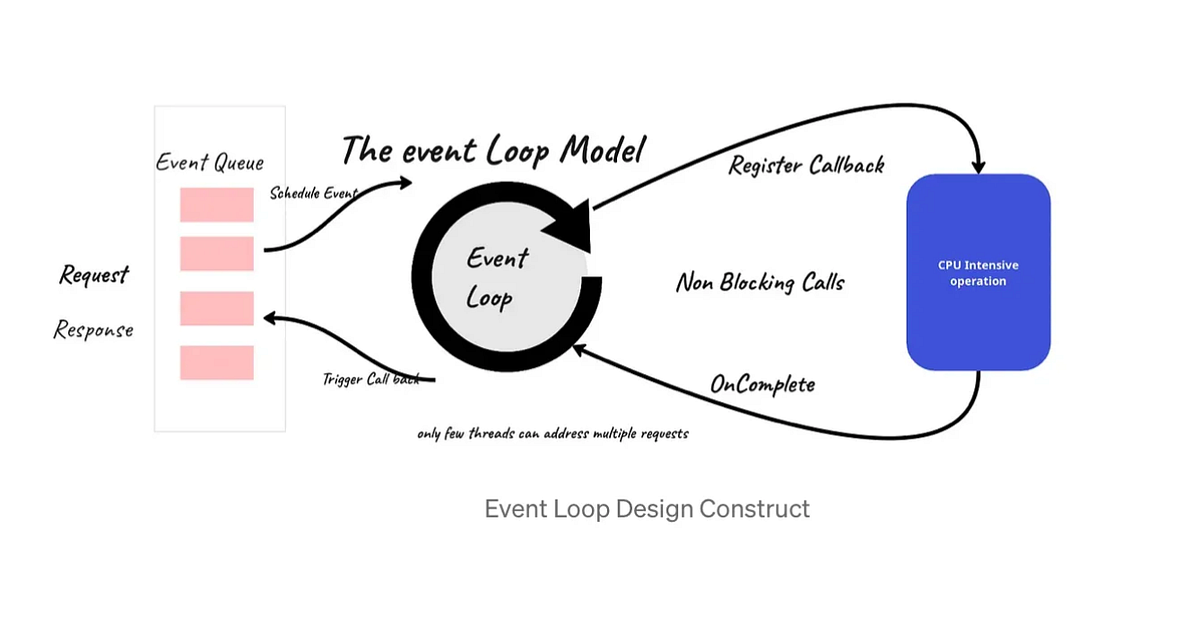
\includegraphics[width=\linewidth,height=0.52\textheight,keepaspectratio]{event-loop-model.png}
    \caption{Event loop: the main loop launches workers; workers return asynchronously.}
\end{figure}

Why asynchronous? Two classic cases:
\begin{itemize}
    \item \textbf{Network}: many connections, each I/O may block for a long and unpredictable time; while one is blocked, the CPU can serve others.
    \item \textbf{UI}: blocking the main thread drops frames; a single block is a visible freeze.
\end{itemize}

\section{Event Loop in SGLang}
SGLang's scheduler is a single-threaded event loop with two modes:
\begin{itemize}
    \item \textbf{overlap (async, default)}: the CPU prepares and samples batch $N{+}1$ while the GPU runs batch $N$, via separate CUDA streams.
    \item \textbf{normal (sync)}: the CPU waits for each forward to finish; a fallback used where overlap is unsupported.
\end{itemize}
The CPU still has real per-step work --- scheduling, sampling, and pre/post-processing --- not ``nothing to do''. The overlap scheduler exists to hide exactly this CPU work behind the GPU forward. Speculative decoding is a typical case that amplifies it: a draft-model forward, verification, and accept/reject bookkeeping are added on top of the normal step.

\subsection{Various Parallelism}
To serve a model larger than one GPU, the model or data is sharded along some axis:
\begin{itemize}
    \item \textbf{DP (Data Parallelism)}: shard the batch; each replica serves its own requests independently.
    \item \textbf{TP (Tensor Parallelism)}: shard the hidden dimension; one forward spans all GPUs with all-reduce.
    \item \textbf{EP (Expert Parallelism)}: shard the experts (MoE); tokens are dispatched via all-to-all.
    \item \textbf{PP (Pipeline Parallelism)}: shard the layers; a batch flows through the stages.
\end{itemize}

\end{document}
